\documentclass[11pt]{article}
\usepackage{mypackages}
\begin{document}

% Max 

\section{Experiments}

The aim of this project is to examine the effect of threading
in stability of deep reinforcement learning.
To acheive this we have solved both simple and advanced problems to investigate
the benefits and disadvantages of asynchronous training in two very different
settings.

\subsection{Playing CartPole - Actor-Critic with eligibility traces}

As a proof of concept we have implemented the method described in section
\ref{sec:actor_critic_el} for which the pseudo-code
can be found in appendix \ref{a:pseudo_code_et}.
The goal of this experiment is to show that a 
traditional Reinforcement Learning algorithm
is able to learn how to solve the CartPole problem, as well as provide a
baseline performance for the A3C algorithm.
I.e as a measure to test if A3C is performing at least as good
as the single-threaded Actor-Critic approach.

For this experiment we used two separate neural networks, with no
shared weights, as policy and state-value estimators.
The network that estimates the state-value function consisted of an
input layer with four entries, corresponding to the format of a state in CartPole,
followed by a single hidden layer with eight neurons, and an output layer of a single
neuron.
We used the ReLU to activate the input to the
hidden layer and no activation for the output neuron.

For estimating the policy we used a network with the same structure,
with the only exception being that the output layer consists of two
neurons, each corresponding to the probability of picking an action.
To emulate the probability distribution we used the softmax function
to activate the final layer.

During the implementation of the algorithm, we encountered a problem with
the state-value estimates sometimes becoming too large.
This resulted in both the probabilties of the policy and state-value estimates throwing a \texttt{NaN} error,
meaning they couldn't be represented using the bits they were assigned.
Therefore we had to restrict the parameters of the algorithm to
be small, which might cause the results of the
experiment being at a disadvantage, compared to our A3C implementation, since the learning happend
at a slower pace than could be achieved with a better implementation.

\subsection{Playing CartPole - A3C}

To examine the effect of asynchronous training in a simpler setting than
the Atari games, we have implemented the A3C algorithm presented
in \cite{a3c} and given by the pseudo-code from appendix \ref{a:pseudo_code_a3c}.

We have chosen to also solve the CartPole problem with this approach, as a way to
investigate how asynchronous training influences the stability of the algorithm,
compared to the more traditional Actor-Critic approach, and 
to itself with different amounts of threads.

As in the previous implementation we ecnountered the \texttt{NaN} error,
but to a much lesser degree.
This means that the error should have little to no impact on
the final results.

To estimate the policy and state-value functions we used a single
neural network.
The structure of the network resembles the structure descrubed in the previous section, 
with the key difference being that the network has two output layers -
one output layer for the policy and another for the value.

\begin{figure}[H]
    \centering
    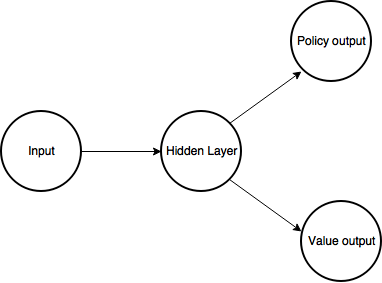
\includegraphics[scale=0.5]{include/shared_cartpole.png}
    \caption{The neural network used to estimate both the state-value
             and policy functions.}
    \label{fig:s_cartpole}
\end{figure}

For both the CartPole problem and the Atari games we will be using the same asynchronous setup
as described in \cite{a3c}.
This means that we will be using a single global network, whose only
purpose is to keep track of a set of global weights, and a local network
for each thread.
To perform the asynchronous update of the global weights we will be using
RMSpropagation as described in section \ref{sec:a3c}.
The parameters of the RMSpropagation, and the algorithm in general, have
been chosen because they provide decent test results.
Due to the time limitations of the project we haven't performed
a more sophisticated selection of the parameters, which might
influence the results of the experiments.

\subsection{Playing Atari Games}

To make sure the advantages and disadvantages of asynchronous training
is thoroughly investigated 
To investigating how the asynchronous training performs in
a more advanced setting, we have also implemented the A3C algorithm
to play Atari games.
We will be examining the effect of different amounts of threads
in Space Invader and Breakout, and compare it to the results
of the Cartpole experiments.

The main difference between this implementation of A3C
and the one we used to play CartPole is the structure of the
policy and value estimator.
We used a single network with two output layers,
based on the setup presented in \cite{dqn-nature}, with the
exception that the input layer of the network takes an $84 \times 84 \times 4$
image-stack as input.
Instead of feeding the network a single frame from the games,
we stack the four latest frames in an attempt to let the network
experience the movement of objects.
This layers is followed by a convolutional layer that reduces the dimensions
of each element in the stack by a factor of four in both dimensions.
Using 16 kernel filters, the layer produces 16 different
$21 \times 21$ feature maps.
In the next layer the size of each of the 16 feature maps is
halved.
This convolution produces 32 new feature maps consisting of $11 \times 11$ values,
using 32 kernel filters.
Both of the convolutional layers activates
their input using the ReLU function.
After the second convolution, we flatten the output.
We perform this step to allow the network to output a numerical value and
probability vector instead of a multichannel matrix.
The flattening results in $3872$ neurons, that are fully connected to
a layer with 256 neurons.
In this layer the input is again activated by a ReLU function,
and the output is sent to two different layers.
One of the layers consists of a single neuron
and simply outputs the weighted sum of its input as the estimated value
of the “state”.
The other output layer activates its input using the softmax function,
with as many neurons as actions available, where
the output of each neuron represents the probability of taking an action.
A representation of the network is shown below.

\begin{figure}[H]
    \centering
    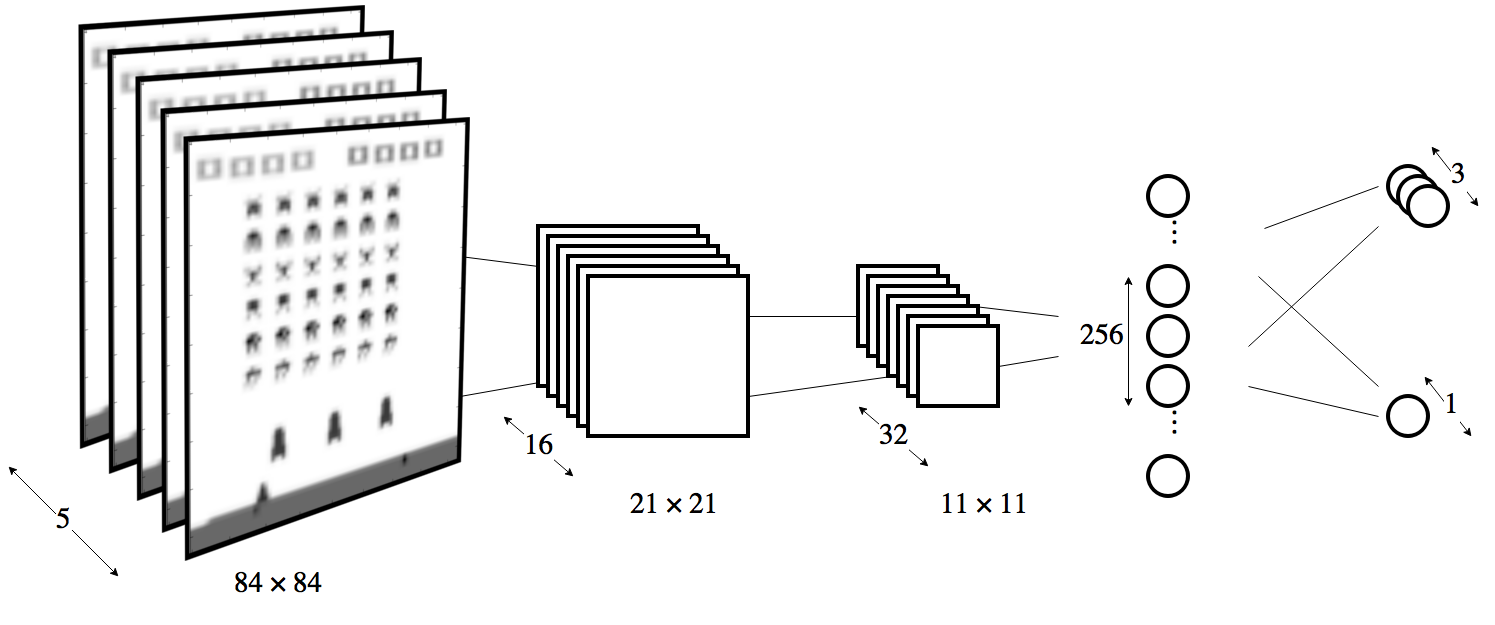
\includegraphics[scale=0.25]{include/Atari_network.png}
    \caption{The neural network used to estimate both the state-value
             and policy functions for Atari games. In this example the network
             is used on Space Invaders which means it has to assign each of three actions a probability.}
    \label{fig:atari_network}
\end{figure}

Taking an action using the OpenAI framework only leads to a relatively small state change,
since it is only performed for two to four frames.
To increase the impact of taking an action we have used the same \textit{action repeat}
stategy as described in \cite{a3c}, which means that an action is performed four times
after being sampled.
We only consider the fourth frame as the one the action produced, but we accumulate the rewards that
we are given during the action repeat, since they are a product of the action.

In Space Invaders we perform two additional preprocessing steps before
the states are fed to the network.
The obtainable rewards vary based on which aliens the learning agent
hits.
The optimal strategy is however to shoot all aliens in a level, and not focus on
shooting only the ones that produce the greatest reward.
Therefore we have chosen to clip the rewards returned by the environment, such that
the rewards always lie between $-1$ and $1$, with the expectation that it should increase
the pace of the learning.
The other issue in Space Invaders is that the screen sometimes flicker.
This can cause the the frame to be missing some objects, and
to avoid this issue we always define a state as the pixel-wise maximum
between the previous frame and the current frame.

\end{document}
